\documentclass[conference]{IEEEtran}
\usepackage{amsmath,booktabs,graphicx}

\title{Comparing Attention-Pooled Recurrent Networks for IMDb Sentiment Classification}

\author{
\IEEEauthorblockN{Nicholas Ampimah, Yin Po Po Aung, and Jane Ohia}
\IEEEauthorblockA{ CSCE 879 - Introduction to Deep Learning}
}

\begin{document}
\maketitle

\begin{abstract}
We compare bidirectional gated recurrent unit (BiGRU) and long short-term memory (BiLSTM) encoders for binary sentiment classification of IMDb reviews. Both architectures use learned embeddings, masked attention pooling, and classifier dropout of 0.20 or 0.50, giving four models. A stratified split of the official training set is used for early stopping and model selection, while the official test set remains held out. BiLSTM-A, selected by minimum validation cross-entropy, achieved 84.94\% test accuracy, 0.849 macro-F1, and 15.06\% error with a 95\% Wilson confidence interval of 14.63--15.51\%. Increasing dropout from 0.20 to 0.50 worsened minimum validation loss for both recurrent architectures and did not eliminate overfitting.
\end{abstract}

\begin{IEEEkeywords}
sentiment analysis, IMDb, recurrent neural networks, attention, dropout
\end{IEEEkeywords}

\section{Introduction}
Review sentiment depends on word order and context. Negation can reverse the meaning of a phrase, and a later clause can change the tone of an earlier one. On the IMDb sentiment benchmark \cite{maas}, we compare BiGRU and BiLSTM encoders with the same attention mechanism and classifier head. Within each architecture, only the dropout setting is changed to examine whether stronger regularization improves validation performance and reduces overfitting. BiLSTM-A was selected at validation loss 0.3038 and achieved 84.94\% test accuracy and 0.849 macro-F1. Across the four models, test accuracy varied by 0.99 percentage points, while all four learning curves showed validation deterioration after their best checkpoint. Paired McNemar tests show that BiGRU-A, BiGRU-B, and BiLSTM-A are statistically indistinguishable on the test set, whereas BiLSTM-B is significantly worse.

\section{Problem and Data}
The input is a movie review represented by at most 200 token IDs, and the output is the probability $p_\theta(y=1\mid x)$ that the review is positive, where $y\in\{0,1\}$. A score above 0.5 predicts positive sentiment. Training minimizes binary cross-entropy,
\begin{equation}
\mathcal{L}=-\frac{1}{B}\sum_{i=1}^{B}
[y_i\log p_i+(1-y_i)\log(1-p_i)].
\end{equation}
This objective is appropriate for binary probabilistic classification and penalizes confident incorrect predictions. The fixed 0.5 threshold avoids tuning a decision threshold on the test set.

TensorFlow Datasets supplies 25,000 labeled training and 25,000 test reviews. Using seed 42, the official training set is divided by a stratified split into 20,000 training and 5,000 validation reviews. The official test split remains separate from architecture and hyperparameter selection. Text is lowercased; HTML line breaks and most punctuation are removed, while apostrophes are retained for contractions. The vocabulary contains at most 15,000 entries, including padding and unknown tokens, and is fitted only on the training reviews. Reviews are padded or truncated to 200 tokens to bound computation, although truncation can discard sentiment evidence appearing late in a review.

\section{Architectures and Training}
A learned embedding maps each token to 64 features. The recurrent encoder is either a bidirectional GRU or bidirectional LSTM with 48 units in each direction, producing a $200\times96$ sequence of contextual states. Bidirectionality is appropriate because the full review is available at inference and sentiment can depend on both preceding and following words. GRUs use update and reset gates, while LSTMs use input, forget, and output gates together with a separate cell state.

\begin{table}[!t]
\caption{Architecture comparison. Shapes omit the batch dimension.}
\label{tab:architecture}
\centering
\footnotesize
\setlength{\tabcolsep}{3.5pt}
\begin{tabular}{@{}lll@{}}
\toprule
Stage & BiGRU & BiLSTM\\
\midrule
Token IDs & 200 & 200\\
Embedding & $200\times64$ & $200\times64$\\
Encoder & GRU, 48/direction & LSTM, 48/direction\\
Encoder output & $200\times96$ & $200\times96$\\
Pooling & Masked attention, 96 & Same\\
Classifier & Dense 32, ReLU, dropout & Same\\
Output & Dense 1, sigmoid & Same\\
Parameters & 999,105 & 1,009,665\\
\bottomrule
\end{tabular}
\end{table}

The attention layer computes
\begin{equation}
s_t=v^\top\tanh(Wh_t+b), \qquad
\alpha_t=\frac{\exp(s_t)}{\sum_j\exp(s_j)},
\end{equation}
over nonpadding positions and returns the weighted sum $\sum_t\alpha_t h_t$. It can therefore emphasize informative locations throughout the retained review instead of relying only on the final recurrent state. The pooled vector passes through a 32-unit ReLU layer, dropout, and a sigmoid output. Setting A uses dropout 0.20 and setting B uses 0.50. Dropout serves as the regularizer by discouraging reliance on individual classifier features.

\textbf{[NEW]} Activations and design choices. Recurrent gates use sigmoid and candidate/state updates use tanh (Keras defaults), attention scoring uses tanh, the 32-unit hidden layer uses ReLU, and the output is a sigmoid so the model returns a probability for binary cross-entropy. Dropout, the regularizer, is placed after the dense layer, where the 96-dimensional pooled vector is compressed; 0.20 is a mild baseline and 0.50 the strong end of the usual range, so the two settings bracket the regularization effect. Small hidden sizes (48 units, 64-dimensional embeddings) keep the four-model comparison tractable on 20,000 training reviews, and early stopping on validation loss rather than accuracy also penalizes overconfident errors. The hyperparameters are: dropout 0.20/0.50, 48 units per direction, 64-dimensional embeddings, vocabulary 15,000, length 200, Adam at $10^{-3}$, batch size 128, patience 5, seed 42.

All models use Adam with learning rate $10^{-3}$ and batch size 128. Early stopping monitors validation loss with patience 5 and restores the minimum-validation-loss checkpoint. The actual run used a 300-epoch safety cap, but all models stopped after the required five-epoch non-improvement window. The winning model was fixed using validation loss before the official test set was evaluated.

\begin{table*}[!t]
\caption{Held-out performance. Validation loss is measured at the best checkpoint. $^\ast$Selected by validation loss. Error intervals are 95\% Wilson confidence intervals.}
\label{tab:results}
\centering
\small
\setlength{\tabcolsep}{4.2pt}
\begin{tabular}{lrrrrrrr}
\toprule
Model & Best/Stop & Val. Loss & Accuracy (\%) & Macro-F1 & ROC AUC & Error (\%) & Error CI (\%)\\
\midrule
BiGRU-A & 2/7 & 0.3040 & 85.06 & 0.850 & 0.931 & 14.94 & [14.51, 15.39]\\
BiGRU-B & 2/7 & 0.3055 & 85.10 & 0.851 & 0.930 & 14.90 & [14.47, 15.35]\\
BiLSTM-A$^\ast$ & 2/7 & \textbf{0.3038} & 84.94 & 0.849 & 0.930 & 15.06 & [14.63, 15.51]\\
BiLSTM-B & 2/7 & 0.3170 & 84.11 & 0.841 & 0.927 & 15.89 & [15.44, 16.35]\\
\bottomrule
\end{tabular}
\end{table*}

\section{Held-Out Results}
\subsection{Metrics and Confidence Intervals}
Accuracy summarizes correct classifications, macro-F1 gives equal weight to the two classes, and ROC AUC evaluates probability ranking across thresholds. For $k$ errors among $n$ held-out reviews, the observed generalization error is $\hat e=k/n=1-\mathrm{accuracy}$. The 95\% Wilson interval used in the analysis is
\begin{equation}
\frac{\hat e+z^2/(2n)\ \pm\ z
\sqrt{\hat e(1-\hat e)/n+z^2/(4n^2)}}
{1+z^2/n},
\end{equation}
where $z=1.96$. This interval quantifies test-sample uncertainty conditional on the fitted model; it does not measure retraining variability, dataset shift, or paired differences between models.

\textbf{[NEW]} For a paired comparison of two models on the same $n$ test reviews, let $b$ be the number classified correctly only by model A and $c$ the number classified correctly only by model B. The accuracy difference is $(b-c)/n$ with 95\% interval $(b-c)/n\pm1.96\sqrt{b+c-(b-c)^2/n}\,/n$, and McNemar's exact test gives a $p$-value from a binomial test of $b$ out of $b+c$ with probability 0.5.

\subsection{Model Selection}
BiLSTM-A had the lowest validation loss (0.3038), narrowly ahead of BiGRU-A (0.3040), and was therefore selected before test evaluation. BiGRU-B had the highest observed test accuracy (85.10\%), but its validation loss was worse (0.3055). Because architecture and hyperparameter selection are part of training, the test ranking is descriptive and cannot be used retroactively to replace the validation-selected model. The individual confidence intervals of BiGRU-A, BiGRU-B, and BiLSTM-A overlap substantially and do not establish statistically significant paired differences between them. \textbf{[NEW]} Because overlapping intervals are only an indirect check, we also compared models on the same 25,000 test reviews with McNemar's exact test (Table~\ref{tab:paired}). BiGRU-A, BiGRU-B, and BiLSTM-A are not significantly different from one another ($p=0.28$--$0.77$), whereas BiLSTM-B is 0.8--1.0 points less accurate than each of them ($p<10^{-4}$).

\begin{table}[!t]
\caption{\textbf{[NEW]} Paired test-set comparison: accuracy difference (A $-$ B) with 95\% CI and McNemar $p$.}
\label{tab:paired}
\centering
\footnotesize
\setlength{\tabcolsep}{3pt}
\begin{tabular}{@{}llr@{}}
\toprule
Model A vs.\ B & Diff.\ (pts) [95\% CI] & $p$\\
\midrule
BiGRU-A vs.\ BiGRU-B & $-0.04$ [$-0.29$, $+0.21$] & 0.77\\
BiGRU-A vs.\ BiLSTM-A & $+0.12$ [$-0.14$, $+0.38$] & 0.37\\
BiGRU-A vs.\ BiLSTM-B & $+0.94$ [$+0.61$, $+1.27$] & $<10^{-4}$\\
BiGRU-B vs.\ BiLSTM-A & $+0.16$ [$-0.12$, $+0.44$] & 0.28\\
BiGRU-B vs.\ BiLSTM-B & $+0.98$ [$+0.66$, $+1.31$] & $<10^{-4}$\\
BiLSTM-A vs.\ BiLSTM-B & $+0.82$ [$+0.49$, $+1.16$] & $<10^{-4}$\\
\bottomrule
\end{tabular}
\end{table}

\begin{figure*}[!t]
\centering
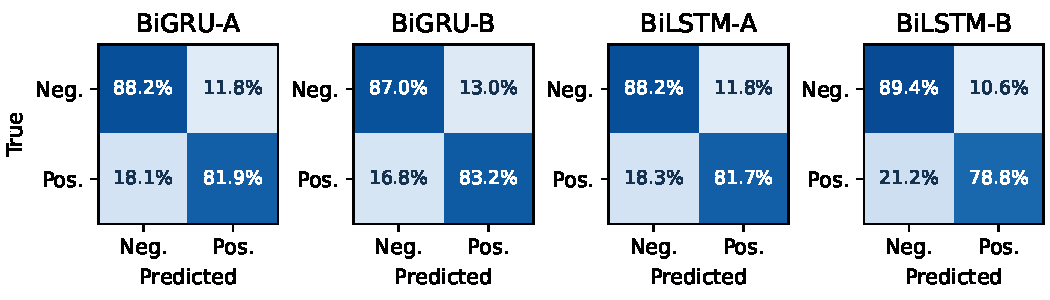
\includegraphics[width=.92\textwidth]{results/confusion_matrices.pdf}
\caption{Row-normalized test confusion matrices. Rows are true classes, columns are predicted classes, and diagonal entries are class recalls.}
\label{fig:cm}
\end{figure*}

\subsection{Class-Specific Performance}
Figure~\ref{fig:cm} gives the required normalized confusion matrices. False positives are negative reviews predicted positive, while false negatives are positive reviews predicted negative. Every model missed more positive reviews than negative reviews. BiLSTM-A produced 2,288 false negatives and 1,478 false positives, corresponding to 81.70\% positive recall and 88.18\% negative recall. Because the test set is balanced, overall accuracy is the average of the two class recalls.

\begin{figure*}[!t]
\centering
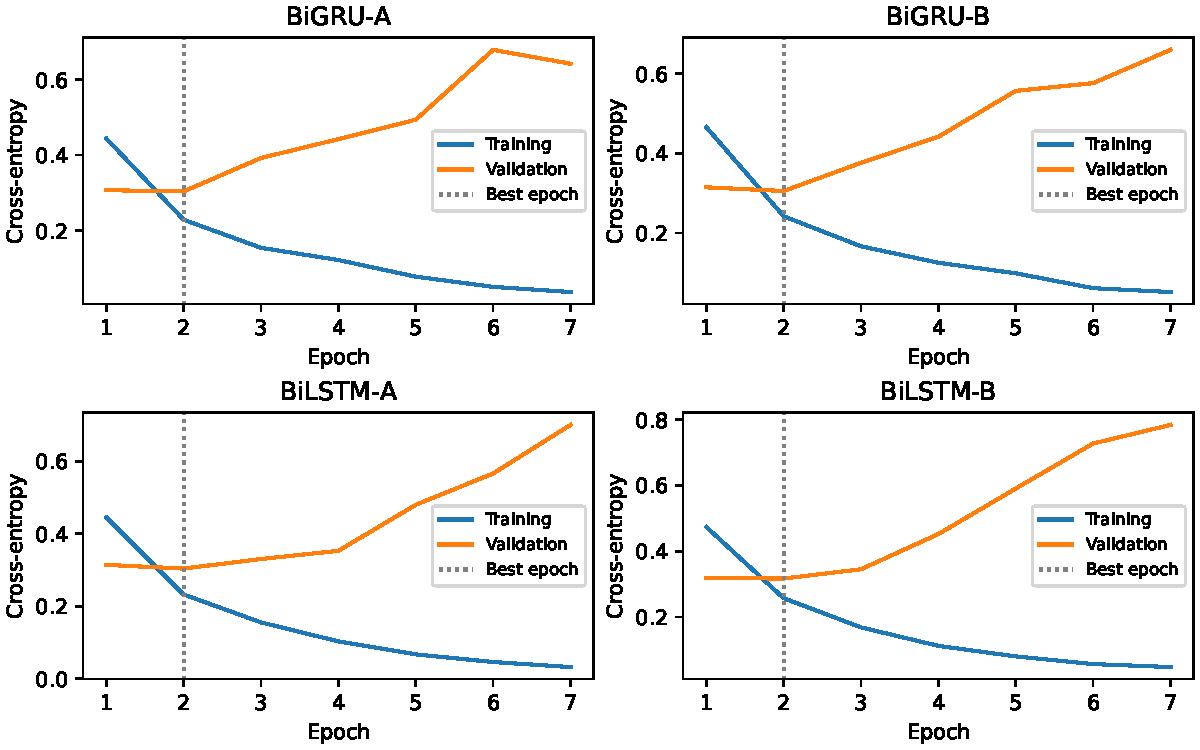
\includegraphics[width=.78\textwidth]{results/learning_curves.pdf}
\caption{Binary cross-entropy by epoch. Vertical lines mark each model's best validation checkpoint.}
\label{fig:curves}
\end{figure*}

\section{Dropout and Overfitting}
The assignment requires discussion of the impact of the regularizer and of overfitting. Figure~\ref{fig:curves} provides direct evidence by comparing training and validation cross-entropy across epochs. Falling training loss accompanied by rising validation loss indicates that continued fitting improves the training objective while harming validation performance.

Increasing dropout from 0.20 to 0.50 changed minimum validation loss from 0.3040 to 0.3055 for BiGRU and from 0.3038 to 0.3170 for BiLSTM, so stronger dropout did not improve validation performance in either architecture. For BiGRU, the best-epoch validation-minus-training loss gap narrowed from 0.0750 to 0.0635, yet validation loss still increased. This smaller gap alone is not sufficient evidence of improved generalization because dropout is active while training loss is measured. For BiLSTM, both settings reached their minimum validation loss at epoch 2, and the gap likewise narrowed from 0.0716 to 0.0598 without improving validation loss. On the test set, dropout 0.50 made no significant difference for BiGRU (85.06\% versus 85.10\%) but reduced BiLSTM accuracy from 84.94\% to 84.11\% ($p<10^{-4}$).

All four models continued to reduce training loss after their best validation checkpoint while validation loss ultimately rose. For BiLSTM-A, training loss decreased from 0.2322 at epoch 2 to 0.0320 at epoch 7 while validation loss increased from 0.3038 to 0.7004. Thus, dropout 0.50 did not eliminate overfitting, and early stopping was important for retaining the best-generalizing checkpoint.

\section{Strengths and Limitations}
The shared prediction head, identical data split, common optimizer settings, and one-factor dropout comparison support a controlled comparison. Fitting the vocabulary only on the training data and fixing the winner before test evaluation reduce leakage. Normalized confusion matrices and confidence intervals provide more information than accuracy alone.

There are also limitations. The encoders have different parameter counts, so observed differences cannot be attributed solely to GRU versus LSTM gate design. Only one split and one seed were used, which limits claims about retraining variability. \textbf{[NEW]} Indeed, an earlier run of the same code reproduced the BiGRU results exactly but gave different BiLSTM results (e.g., 85.15\% test accuracy for BiLSTM-B), so small BiLSTM differences should not be over-interpreted. Truncating reviews to 200 tokens and capping the vocabulary improve computational tractability but may remove useful sentiment evidence. Attention weights indicate where the model places emphasis but do not constitute causal explanations. Finally, the conclusions apply to polarized IMDb movie reviews and do not establish performance on neutral sentiment or other domains.

\section{Conclusion}
BiLSTM-A was selected by minimum validation cross-entropy and achieved 84.94\% test accuracy, 0.849 macro-F1, and 15.06\% error with a 95\% Wilson confidence interval of 14.63--15.51\%. BiGRU-A, BiGRU-B, and BiLSTM-A produced statistically indistinguishable held-out accuracy, while BiLSTM-B was significantly worse. Increasing dropout to 0.50 did not improve minimum validation loss for either recurrent architecture, and all four models showed overfitting after their best checkpoint. The results therefore support validation-based model selection and early stopping as important components of this sequential sentiment-classification experiment.

\begin{thebibliography}{1}
\bibitem{maas}
A.~L. Maas \emph{et al.}, ``Learning word vectors for sentiment analysis,'' in \emph{Proc. ACL-HLT}, 2011, pp. 142--150.
\end{thebibliography}

\end{document}
